\documentclass[tikz,border=4pt]{standalone}
% Shared TikZ style for lecture figures
\usepackage{amsmath,amssymb}
\usepackage{tikz}
\usetikzlibrary{arrows.meta,calc,decorations.pathreplacing,patterns}
\definecolor{teal}{RGB}{38,150,140}
\definecolor{coral}{RGB}{230,95,75}
\definecolor{ink}{RGB}{20,45,60}
\tikzset{
  >={Stealth[length=2.6mm]},
  every picture/.style={line cap=round,line join=round,thick,ink},
  map/.style={->,thick},
  dot/.style={circle,fill,inner sep=1.2pt},
}

\begin{document}
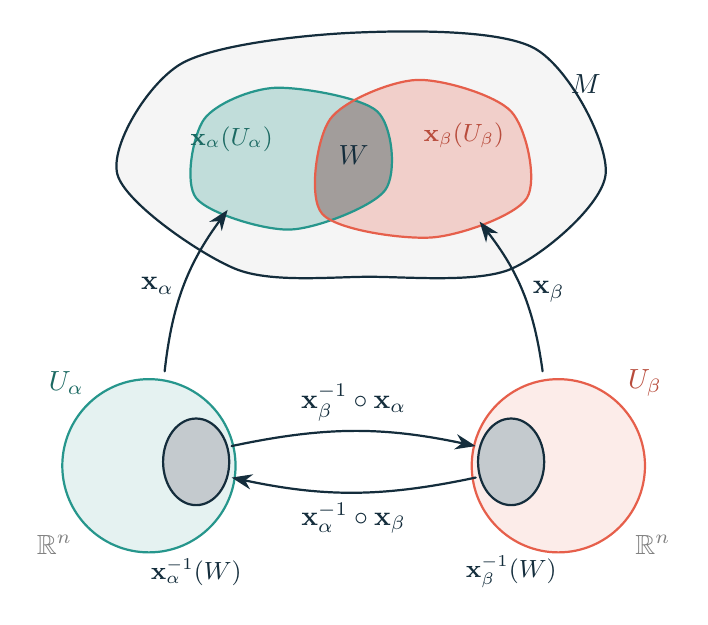
\begin{tikzpicture}
  \def\blobA{plot[smooth cycle] coordinates {(2.0,4.3) (3.2,3.9) (4.4,4.4) (4.3,5.4) (3.0,5.7) (2.1,5.3)}}
  \def\blobB{plot[smooth cycle] coordinates {(3.6,4.1) (5.0,3.8) (6.2,4.3) (6.0,5.4) (4.8,5.8) (3.7,5.3)}}
  % the manifold / surface
  \draw[fill=gray!8] plot[smooth cycle] coordinates {(1.0,4.6) (2.5,3.4) (4.2,3.3) (6.0,3.4) (7.2,4.6) (6.3,6.2) (4.0,6.4) (1.8,6.0)};
  \node at (6.95,5.75) {$M$};
  \fill[teal,opacity=0.25] \blobA;
  \fill[coral,opacity=0.25] \blobB;
  \begin{scope}
    \clip \blobA;
    \fill[ink,opacity=0.22] \blobB;
  \end{scope}
  \draw[teal] \blobA; \draw[coral] \blobB;
  \node at (4.0,4.85) {$W$};
  \node[teal!70!black] at (2.45,5.05) {\small $\mathbf{x}_{\alpha}(U_{\alpha})$};
  \node[coral!80!black] at (5.4,5.1) {\small $\mathbf{x}_{\beta}(U_{\beta})$};
  % parameter domains
  \draw[fill=teal!12,draw=teal] (1.4,0.9) circle (1.1);
  \node[teal!70!black] at (0.35,1.95) {$U_{\alpha}$};
  \draw[fill=ink!25] (2.0,0.95) ellipse (0.42 and 0.55);
  \node at (2.0,-0.45) {\small $\mathbf{x}_{\alpha}^{-1}(W)$};
  \draw[fill=coral!12,draw=coral] (6.6,0.9) circle (1.1);
  \node[coral!80!black] at (7.7,1.95) {$U_{\beta}$};
  \draw[fill=ink!25] (6.0,0.95) ellipse (0.42 and 0.55);
  \node at (6.0,-0.45) {\small $\mathbf{x}_{\beta}^{-1}(W)$};
  \node[gray] at (0.2,-0.1) {$\mathbb{R}^{n}$};
  \node[gray] at (7.8,-0.1) {$\mathbb{R}^{n}$};
  % maps
  \draw[map] (1.6,2.1) to[bend left=15] node[left] {$\mathbf{x}_{\alpha}$} (2.4,4.15);
  \draw[map] (6.4,2.1) to[bend right=15] node[right] {$\mathbf{x}_{\beta}$} (5.6,4.0);
  \draw[map] (2.45,1.15) to[bend left=12] node[above] {$\mathbf{x}_{\beta}^{-1}\circ\mathbf{x}_{\alpha}$} (5.55,1.15);
  \draw[map] (5.55,0.75) to[bend left=12] node[below] {$\mathbf{x}_{\alpha}^{-1}\circ\mathbf{x}_{\beta}$} (2.45,0.75);
\end{tikzpicture}
\end{document}
